\chapter{Obetivos o Introduccion}
    \pagenumbering{arabic}
    \section{SEccion 1}
    Para poder usar la maquina virtual "LAMP" que se encuentra en aulas, primero debemos descargar el programa VirtualBox desde \url{https://www.virtualbox.org/wiki/Downloads}.
    
    Luego tenemos que obtener la mencionada maquina virtual desde la web del curso, que se encuentra en \url{https://aulas.ort.edu.uy/course/view.php?id=3885&section=10} .
    Dependiendo de la arquitectura de su OS debe bajar el archivo de 32bits o 64bits.
    
    Descargada la VM(virtual machine) se debe agregar a la aplicación de VirtualBox, haciéndolo desde el menú o dándole doble click al archivo. Hecho esto se debería de ver como la siguiente imagen:
    \begin{figure} [H]
            \centering
            \frame{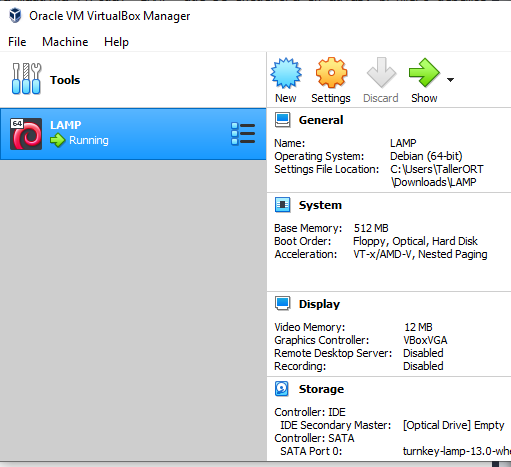
\includegraphics[width=4in]{imagen/vm1.png}}
            \caption{Inicio de VirtualBox}
    \end{figure}
    
    \clearpage
    Tenemos que iniciar LAMP con el botón de la flecha verde. Con esto nos cargara una pantalla donde se muestra el sistema operativo Linux iniciando, y al terminar nos mostrara la dirección ip que se usara para cada servicio.
    
    A continuación se despliega una muestra de como se vería:
    
    \begin{figure} [H]
            \centering
            \frame{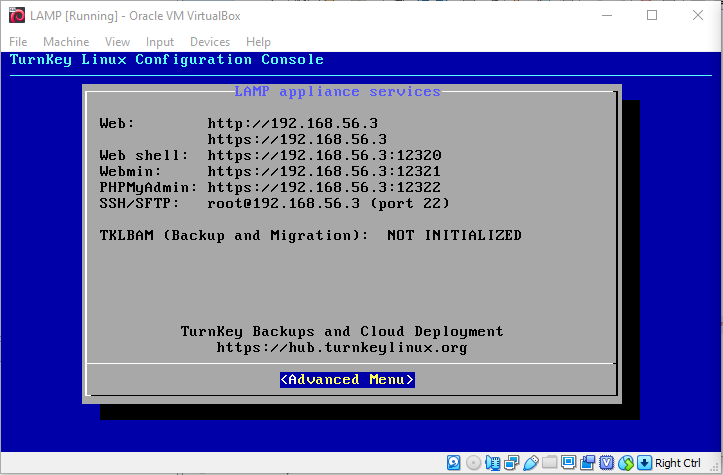
\includegraphics[width=4in]{imagen/vm2.png}}
            \caption{Maquina virtual corriendo}
    \end{figure}
    
    
    Con esta IP ya podemos acceder desde cualquier navegador a la configuracion tanto de la bases de datos en Mysql como del linux y dentro de este del servidor Apache con PHP.
    \clearpage
    Al acceder veremos lo siguiente:
    \begin{figure} [H]
            \centering
            \frame{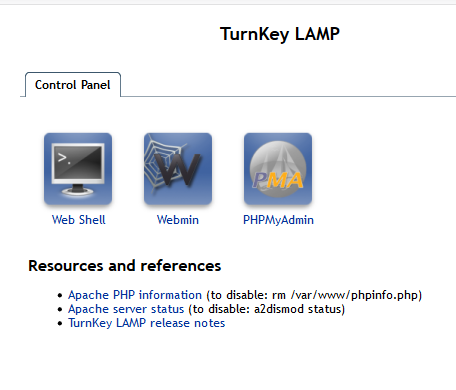
\includegraphics[width=4in]{imagen/IP.png}}
            \caption{Acceso por navegador}
    \end{figure}
    
    Tanto para acceder a la consola como al administrador de Mysql es necesario usar las credenciales: usuario= root, password = root.
    Si queremos acceder al Linux por otra via que no sea "Web Shell" también se puede usar putty. Lo mismo para subir archivos, podemos hacerlo con la app WinSCP.
    
\chapter{Fuentes}
    \pagenumbering{arabic}
    \section{Acceso a las fuentes}
    Todas las fuentes de este obligatorio están accesibles en
    \url{https://app.box.com/s/redahk46upihnq7uaryd1gdcpwt29c92}
